
\chapter{Kronecker and Vec Operator}

\section{Flattening}

Flattening is a common operation for programmers.
In the language of numpy, we may write
\verb|np.ones((2,3,4)).reshape(2, 12)| to flatten a shape (2,3,4) tensor into a shape (2,12) matrix.
Similarly, in mathematical notation, $\mathrm{vec}(X)$ is commonly used to denote the flattening of a matrix into a vector.

Typically the main reason to do this is as a cludge for dealing with bad general notation for tensors.
Hence, with tensor diagrams, we can avoid this operation entirely.
However, it is still interesting to see how tensor diagrams can make a lot of properties of flattening much more transparent.

To begin with we note that flattening is a linear operation, and hence can be represented as a simple tensor.
We'll use a triangle to denote this:
\[
   \triangleright_{i,j,k}=
\begin{tikzpicture}[baseline=-.25em]
\node[triangle] (c0) at (1.5,0) {};
\draw (c0) -- ++(-.5, .5) node[midway, above right, font=\tiny] {i};
\draw (c0) -- ++(-.5, -.5) node[midway, above left, font=\tiny] {j};
\draw[double] (c0) -- ++(.5, 0) node[midway, above, font=\tiny] {k};
\end{tikzpicture}
= [i + j n = k]
.
\]
Here $n$ is the dimension of the $i$ edge.
Note we use a double line to denote the output of the flattening operation.
This is simply a syntactic choice to remind ourselves that the output is a bundle of two edges.

Using this notation we can write
\[
   \mathrm{vec}(X)_k
   = \sum_{i,j} \triangleright_{i,j,k} X_{i,j}
   =
   \begin{tikzpicture}[baseline=-.25em]
      \node (X) at (.5,0) {X};
      \node[triangle] (c0) at (1.5,0) {};
      \draw (X) edge[bend left] (c0);
      \draw (X) edge[bend right] (c0);
      \draw[double] (c0) -- ++(.5, 0) node[midway, above, font=\tiny] {k};
   \end{tikzpicture}
   .
\]
The basic property of $\triangleright$ is that opposing triangles cancel:
\begin{align}
\begin{tikzpicture}[baseline=-.3em]
\node (X) at (.5,0) {\phantom{X}};
\node[triangle] (c0) at (1.5,0) {};
\node[triangle, rotate=180] (c1) at (2.5,0) {};
\node (Y) at (3.5,0) {\phantom{Y}};
\draw (X) edge[bend left] (c0);
\draw (X) edge[bend right] (c0);
\draw[double] (c0) -- (c1);
\draw (Y) edge[bend left] (c1);
\draw (Y) edge[bend right] (c1);
\end{tikzpicture}
&=
\begin{tikzpicture}[baseline=-.3em]
\node (X) at (0,0) {\phantom{X}};
\node (Y) at (1.5,0) {\phantom{Y}};
\draw (X) edge[bend left] (Y);
\draw (X) edge[bend right] (Y);
\end{tikzpicture}
\\\text{and}
\begin{tikzpicture}[baseline=-.3em]
\node (X) at (.5,0) {\phantom{X}};
\node[triangle, rotate=180] (c0) at (1.5,0) {};
\node[triangle] (c1) at (2.5,0) {};
\node (Y) at (3.5,0) {\phantom{Y}};
\draw[double] (X) -- (c0);
\draw (c0) edge[bend left] (c1);
\draw (c0) edge[bend right] (c1);
\draw[double] (Y) -- (c1);
\end{tikzpicture}
&=
\begin{tikzpicture}[baseline=-.3em]
\node (X) at (0,0) {\phantom{X}};
\node (Y) at (1.5,0) {\phantom{Y}};
\draw[double] (X) -- (Y);
\end{tikzpicture}
.
\end{align}
It's also easy to convince oneself of the following ``mixed'' property:
\begin{align}
   \begin{tikzpicture}[baseline=-.25em, inner sep=0pt]
      \node (F0) at (0,0) {$\sbullet$};
      \node[triangle, rotate=180, inner sep=3pt] (Fab0) at (.5,.25) {};
      \node (A) at (1,.333) {};
      \node (B) at (1,.166) {};
      \node[triangle, rotate=180, inner sep=3pt] (Fcd0) at (.5,-.25) {};
      \node (C) at (1,-.166) {};
      \node (D) at (1,-.333) {};
      \draw[double] (F0) -- ++(-.4,0);
      \draw[double] (F0) -- (Fab0);
      \draw[double] (F0) -- (Fcd0);
      \draw (Fab0) -- (A);
      \draw (Fab0) -- (B);
      \draw (Fcd0) -- (C);
      \draw (Fcd0) -- (D);
   \end{tikzpicture}
     \quad=\quad
   \begin{tikzpicture}[baseline=-.25em, inner sep=0pt]
      \node[triangle, rotate=180, inner sep=3pt] (F0) at (0,0) {};
      \node (Fab0) at (.5,.25) {$\sbullet$};
      \node (A) at (1,.333) {};
      \node (B) at (1,.166) {};
      \node (Fcd0) at (.5,-.25) {$\sbullet$};
      \node (C) at (1,-.166) {};
      \node (D) at (1,-.333) {};
      \draw[double] (F0) -- ++(-.4,0);
      \draw (F0) -- (Fab0);
      \draw (F0) -- (Fcd0);
      \draw (Fab0) -- (A);
      \draw (Fab0) -- (C.west);
      \draw (Fcd0) -- (B.west);
      \draw (Fcd0) -- (D);
   \end{tikzpicture}
   \label{eq:flatten_mix}
\end{align}


\section{The Kronecker Product}
The Kronecker product of an $m\times n$ matrix $A$ and an $r \times q$ matrix $B$, is an $mr \times nq$ matrix, $A \otimes B$ defined as
\[
   \renewcommand*{\arraystretch}{1.3}
   A \otimes B = \begin{bmatrix}
      A_{1,1} B & A_{1,2} B & \cdots & A_{1,n} B \\
      A_{2,1} B & A_{2,2} B & \cdots & A_{2,n} B \\
      \vdots & \vdots & \ddots & \vdots \\
      A_{m,1} B & A_{m,2} B & \cdots & A_{m,n} B
   \end{bmatrix}
   .
\]
Using index notation we can also write this as
$(A\otimes B)_{p(r-1)+v, q(s-1)+w} = A_{rs} B_{vw}$, but it's pretty hard to read.

In tensor notation the Kronecker Product is simply the outer product of two matrices, flattened ``on both sides'':
$A\otimes B=$
\begin{tikzpicture}[baseline=-.25em]
   \node[triangle, rotate=180] (F0) at (0,0) {};
   \node (A) at (.6,.25) {A};
   \node (B) at (.6,-.25) {B};
   \node[triangle] (F1) at (1.2,0) {};
   \draw[double] (F0) -- ++(-.4,0);
   \draw[double] (F1) -- ++(.4,0);
   \draw (F0) -- (A) -- (F1);
   \draw (F0) -- (B) -- (F1);
\end{tikzpicture}
.

The Kronecker product has the following properties:
\noindent
%\makebox[\textwidth]{\parbox{1.1\textwidth}{%
\begin{align*}
   \tag{506}
   A \otimes (B + C) &= A \otimes B + A \otimes C
                     &
   \begin{tikzpicture}[baseline=-.25em]
      \node[triangle, rotate=180] (F0) at (0,0) {};
      \node (A) at (1,.25) {A};
      \node (B) at (1,-.25) {(B+C)};
      \node[triangle] (F1) at (2,0) {};
      \draw[double] (F0) -- ++(-.4,0);
      \draw[double] (F1) -- ++(.4,0);
      \draw (F0) -- (A) -- (F1);
      \draw (F0) -- (B) -- (F1);
   \end{tikzpicture}
                     &=
   \begin{tikzpicture}[baseline=-.25em]
      \node[triangle, rotate=180] (F0) at (0,0) {};
      \node (A) at (.6,.25) {A};
      \node (B) at (.6,-.25) {B};
      \node[triangle] (F1) at (1.2,0) {};
      \draw[double] (F0) -- ++(-.4,0);
      \draw[double] (F1) -- ++(.4,0);
      \draw (F0) -- (A) -- (F1);
      \draw (F0) -- (B) -- (F1);
   \end{tikzpicture}
                   \\&&&+
   \begin{tikzpicture}[baseline=-.25em]
      \node[triangle, rotate=180] (F0) at (0,0) {};
      \node (A) at (.6,.25) {A};
      \node (B) at (.6,-.25) {C};
      \node[triangle] (F1) at (1.2,0) {};
      \draw[double] (F0) -- ++(-.4,0);
      \draw[double] (F1) -- ++(.4,0);
      \draw (F0) -- (A) -- (F1);
      \draw (F0) -- (B) -- (F1);
   \end{tikzpicture}
   \\
   \tag{508}
   A \otimes (B \otimes C) &= (A \otimes B) \otimes C
                     &
   \begin{tikzpicture}[baseline=-.25em]
      \node[triangle, rotate=180] (F0) at (0,0) {};
      \node (A) at (1,.333) {A};
      \node[triangle] (F1) at (2,0) {};
      \node (B) at (1,0) {B};
      \node (C) at (1,-.333) {C};
      \node[triangle, rotate=180] (F2) at (.5,-.167) {};
      \node[triangle] (F3) at (1.5,-.167) {};
      \draw[triple] (F0) -- ++(-.4,0);
      \draw[triple] (F1) -- ++(.4,0);
      \draw (F0) -- (A) -- (F1);
      \draw[double] (F0) -- (F2);
      \draw[double] (F3) -- (F1);
      \draw (F2) -- (B) -- (F3);
      \draw (F2) -- (C) -- (F3);
   \end{tikzpicture}
                     &=
   \begin{tikzpicture}[baseline=-.25em]
      \node[triangle, rotate=180] (F0) at (0,0) {};
      \node (A) at (.6,.333) {A};
      \node[triangle] (F1) at (1.2,0) {};
      \node (B) at (.6,0) {B};
      \node (C) at (.6,-.333) {C};
      \draw[triple] (F0) -- ++(-.4,0);
      \draw[triple] (F1) -- ++(.4,0);
      \draw (F0) -- (A) -- (F1);
      \draw (F0) -- (B) -- (F1);
      \draw (F0) -- (C) -- (F1);
   \end{tikzpicture}
                  \\ &&&=
   \begin{tikzpicture}[baseline=-.25em]
      \node[triangle, rotate=180] (F0) at (0,0) {};
      \node (A) at (1,.333) {A};
      \node[triangle] (F1) at (2,0) {};
      \node (B) at (1,0) {B};
      \node (C) at (1,-.333) {C};
      \node[triangle, rotate=180] (F2) at (.5,.167) {};
      \node[triangle] (F3) at (1.5,.167) {};
      \draw[triple] (F0) -- ++(-.4,0);
      \draw[triple] (F1) -- ++(.4,0);
      \draw (F2) -- (A) -- (F3);
      \draw[double] (F0) -- (F2);
      \draw[double] (F3) -- (F1);
      \draw (F2) -- (B) -- (F3);
      \draw (F0) -- (C) -- (F1);
   \end{tikzpicture}
   \\
   \tag{509}
   a A \otimes b B &= a b (A \otimes B)
   &
   \begin{tikzpicture}[baseline=-.25em]
      \node[triangle, rotate=180] (F0) at (0,0) {};
      \node (A) at (.6,.25) {a A};
      \node (B) at (.6,-.25) {b B};
      \node[triangle] (F1) at (1.2,0) {};
      \draw[double] (F0) -- ++(-.4,0);
      \draw[double] (F1) -- ++(.4,0);
      \draw (F0) -- (A) -- (F1);
      \draw (F0) -- (B) -- (F1);
   \end{tikzpicture}
   &=
   \begin{tikzpicture}[baseline=-.25em]
      \node at (-.1,.4) {ab};
      \node[triangle, rotate=180] (F0) at (0,0) {};
      \node (A) at (.6,.25) {A};
      \node (B) at (.6,-.25) {B};
      \node[triangle] (F1) at (1.2,0) {};
      \draw[double] (F0) -- ++(-.4,0);
      \draw[double] (F1) -- ++(.4,0);
      \draw (F0) -- (A) -- (F1);
      \draw (F0) -- (B) -- (F1);
   \end{tikzpicture}
   \\
   \tag{510}
   (A \otimes B)^T &= A^T \otimes B^T
                   &
      \begin{tikzpicture}[baseline=-.25em]
         \node[triangle, rotate=180, minimum size=1cm] (F0) at (0,0) {};
         \node (A) at (.6,.25) {A};
         \node (B) at (.6,-.25) {B};
         \node[triangle, minimum size=1cm] (F1) at (1.2,0) {};
         \draw (F0) -- (A) -- (F1);
         \draw (F0) -- (B) -- (F1);
         \draw[double] (F0) .. controls (-1,0) and (.6,1) .. (2,0);
         \draw[double] (F1) .. controls (2.2,0) and (.6,-1) .. (-.8,0);
      \end{tikzpicture}
                   &=
      \begin{tikzpicture}[baseline=-.25em]
         \node[triangle, rotate=180, minimum size=1cm] (F0) at (-1,0) {};
         \node (A) at (0,.25) {A};
         \node (B) at (0,-.25) {B};
         \node[triangle, minimum size=1cm] (F1) at (1,0) {};
         \draw[double] (F0) -- ++(-.4,0);
         \draw[double] (F1) -- ++(.4,0);
         \draw (A.east) .. controls (1,.1) and (0,0) .. (F0);
         \draw (A.west) .. controls (-1,.5) and (0,.5) .. (F1);
         \draw (B.east) .. controls (1,-.5) and (0,-.5) .. (F0);
         \draw (B.west) .. controls (-1,-.1) and (0,0) .. (F1);
      \end{tikzpicture}
   \\
   \tag{511}
   (A \otimes B)(C \otimes D) &= AC \otimes BD
                              &
   \begin{tikzpicture}[baseline=-.25em]
      \node[triangle, rotate=180] (F0) at (0,0) {};
      \node (A) at (.6,.25) {A};
      \node (B) at (.6,-.25) {B};
      \node[triangle] (F1) at (1.2,0) {};
      \draw[double] (F0) -- ++(-.4,0);
      \draw[double] (F1) -- ++(.4,0);
      \draw (F0) -- (A) -- (F1);
      \draw (F0) -- (B) -- (F1);
      %
      \node[triangle, rotate=180] (F2) at (1.8,0) {};
      \node (C) at (2.4,.25) {C};
      \node (D) at (2.4,-.25) {D};
      \node[triangle] (F3) at (3,0) {};
      \draw (F2) -- (C) -- (F3);
      \draw (F2) -- (D) -- (F3);
      %
      \draw[double] (F1) -- (F2);
      \draw[double] (F3) -- ++(.4,0);
   \end{tikzpicture}
                              &=
   \begin{tikzpicture}[baseline=-.25em]
      \node[triangle, rotate=180] (F0) at (0,0) {};
      \node (A) at (.5,.25) {A};
      \node (B) at (.5,-.25) {B};
      \node (C) at (1.1,.25) {C};
      \node (D) at (1.1,-.25) {D};
      \node[triangle] (F1) at (1.6,0) {};
      \draw[double] (F0) -- ++(-.4,0);
      \draw[double] (F1) -- ++(.4,0);
      \draw (F0) -- (A) -- (C) -- (F1);
      \draw (F0) -- (B) -- (D) -- (F1);
   \end{tikzpicture}
   \\
   \tag{511b}
   (A \otimes I) (I \otimes B) &= A \otimes B
               &
   \begin{tikzpicture}[baseline=-.25em]
      \node[triangle, rotate=180] (F0) at (0,0) {};
      \draw[double] (F0) -- ++(-.4,0);
      \node (A) at (.6,.25) {A};
      \node[triangle] (F1) at (1.2,0) {};
      \draw (F0) -- (A) -- (F1);
      \draw (F0) edge[bend right] (F1);
      %
      \node[triangle, rotate=180] (F2) at (1.8,0) {};
      \node (D) at (2.4,-.25) {B};
      \node[triangle] (F3) at (3,0) {};
      \draw (F2) edge[bend left] (F3);
      \draw (F2) -- (D) -- (F3);
      %
      \draw[double] (F1) -- (F2);
      \draw[double] (F3) -- ++(.4,0);
   \end{tikzpicture}
                              &=
   \begin{tikzpicture}[baseline=-.25em]
      \node[triangle, rotate=180] (F0) at (0,0) {};
      \node (A) at (.6,.25) {A};
      \node (B) at (.6,-.25) {B};
      \node[triangle] (F1) at (1.2,0) {};
      \draw[double] (F0) -- ++(-.4,0);
      \draw[double] (F1) -- ++(.4,0);
      \draw (F0) -- (A) -- (F1);
      \draw (F0) -- (B) -- (F1);
   \end{tikzpicture}
   %\\
   %%\tag{512}
   %(A \otimes B)^{-1} &= A^{-1} \otimes B^{-1} \\
   \\
   \tag{515}
   \mathrm{Tr}(A \otimes B) &= \mathrm{Tr}(A) \mathrm{Tr}(B)
   &
   \hspace{-4em}
   \begin{tikzpicture}[baseline=-.25em]
      \node[triangle, rotate=180] (F0) at (0,0) {};
      \node (A) at (.6,.25) {A};
      \node (B) at (.6,-.25) {B};
      \node[triangle] (F1) at (1.2,0) {};
      \draw (F0) -- (A) -- (F1);
      \draw (F0) -- (B) -- (F1);
      \path (F0) edge [double, out=160, in=20, looseness=4] (F1);
   \end{tikzpicture}
   \hspace{-4em}
   &=
   \hspace{-4em}
   \begin{tikzpicture}[baseline=-.25em]
      \node (A) at (.6,.2) {A};
      \node (B) at (.6,-.2) {B};
      \path (A) edge [out=160, in=20, looseness=2] (A);
      \path (B) edge [out=160, in=20, looseness=11] (B);
   \end{tikzpicture}
   \hspace{-4em}
 \\&&&=
   \vspace{-4em}
   \hspace{-1em}
    \trace{A}{1}
   \hspace{-2em}
    \trace{B}{1}
   \hspace{-1em}
   \\
   \tag{519}
   \hspace{-1cm}
   \mathrm{eig}(A \otimes B) &= \mathrm{eig}(A) \mathrm{eig}(B)
                             &
   \begin{tikzpicture}[baseline=-.25em]
      \node[triangle, rotate=180] (F0) at (0,0) {};
      \node (Q1) at (.6,.25) {$Q_1$};
      \node (Q2) at (.6,-.25) {$Q_2$};
      \node (b1) at (1.25,.25) {$\sbullet$};
      \node (b2) at (1.25,-.25) {$\sbullet$};
      \node (Q1i) at (2,.25) {$Q_1^{-1}$};
      \node (Q2i) at (2,-.25) {$Q_2^{-1}$};
      \node[triangle] (F1) at (2.7,0) {};
      \draw[double] (F0) -- ++(-.4,0);
      \draw[double] (F1) -- ++(.4,0);
      \draw (F0) -- (Q1) -- (b1) -- (Q1i) -- (F1);
      \draw (F0) -- (Q2) -- (b2) -- (Q2i) -- (F1);
      \draw (b1) -- ++(0, .25) node[anchor=south] {$\lambda_1$};
      \draw (b2) -- ++(0, -.25) node[anchor=north] {$\lambda_2$};
   \end{tikzpicture}
                             &=
   \begin{tikzpicture}[baseline=-.25em]
      \node[triangle, rotate=180] (F0) at (0,0) {};
      \node (Q1) at (.55,.25) {$Q_1$};
      \node (Q2) at (.55,-.25) {$Q_2$};
      \node[triangle] (F1) at (1.1,0) {};
      \node[triangle, rotate=180] (F2) at (1.5,0) {};
      \node (b1) at (1.9,.25) {$\sbullet$};
      \node (b2) at (1.9,-.25) {$\sbullet$};
      \node[triangle] (F3) at (2.3,0) {};
      \node[triangle, rotate=180] (F4) at (2.7,0) {};
      \node (Q1i) at (3.35,.25) {$Q_1^{-1}$};
      \node (Q2i) at (3.35,-.25) {$Q_2^{-1}$};
      \node[triangle] (F5) at (4,0) {};
      \draw[double] (F0) -- ++(-.4,0);
      \draw[double] (F5) -- ++(.4,0);
      \draw (F0) -- (Q1) -- (F1);
      \draw (F1) edge[double] (F2);
      \draw (F2) -- (b1) -- (F3);
      \draw (F3) edge[double] (F4);
      \draw (F4) -- (Q1i) -- (F5);
      \draw (F0) -- (Q2) -- (F1);
      \draw (F2) -- (b2) -- (F3);
      \draw (F4) -- (Q2i) -- (F5);
      \draw (b1) -- ++(0, .25) node[anchor=south] {$\lambda_1$};
      \draw (b2) -- ++(0, -.25) node[anchor=north] {$\lambda_2$};
   \end{tikzpicture}
                           \\&&&=
   \begin{tikzpicture}[baseline=-.25em]
      \node[triangle, rotate=180] (F0) at (0,0) {};
      \node (Q1) at (.55,.25) {$Q_1$};
      \node (Q2) at (.55,-.25) {$Q_2$};
      \node[triangle] (F1) at (1.1,0) {};
      \node (b) at (1.9,0) {$\sbullet$};
      \node[triangle, rotate=180] (F4) at (2.7,0) {};
      \node (Q1i) at (3.35,.25) {$Q_1^{-1}$};
      \node (Q2i) at (3.35,-.25) {$Q_2^{-1}$};
      \node[triangle] (F5) at (4,0) {};
      \draw[double] (F0) -- ++(-.4,0);
      \draw[double] (F5) -- ++(.4,0);
      \draw (F0) -- (Q1) -- (F1);
      \draw[double] (F1) -- (b) -- (F4);
      \draw (F4) -- (Q1i) -- (F5);
      \draw (F0) -- (Q2) -- (F1);
      \draw (F4) -- (Q2i) -- (F5);
      \node[triangle, below=.3em of b, rotate=90] (Fb) {};
      \draw[double] (Fb) -- (b);
      \draw (Fb) -- ++(-.1, -.25) node[anchor=north east] {$\lambda_1$};
      \draw (Fb) -- ++(.1, -.25) node[anchor=north west] {$\lambda_2$};
   \end{tikzpicture}
\end{align*}
%}}

Here the last equation shows an interesting general property of $\triangleright$:
\begin{align}
   \begin{tikzpicture}[baseline=-.25em]
      \node[triangle, rotate=180] (F0) at (0,0) {};
      \node (b1) at (.4,.25) {$\sbullet$};
      \node (b2) at (.6,-.25) {$\sbullet$};
      \node[triangle] (F1) at (1,0) {};
      \draw[double] (F0) -- ++(-.4,0);
      \draw[double] (F1) -- ++(.4,0);
      \draw (F0) -- (b1) -- (F1);
      \draw (F0) -- (b2) -- (F1);
      \node (M) at (.3,-.6) {M};
      \draw (M) -- (b1);
      \draw (M) -- (b2);
   \end{tikzpicture}
   =
   \begin{tikzpicture}[baseline=-.25em]
      \node (b) at (.5,0) {$\sbullet$};
      \draw[double] (b) -- ++(-.4,0);
      \draw[double] (b) -- ++(.4,0);
      \node[triangle, rotate=90] (F) at (.5,-.5) {};
      \draw[double] (F) -- (b);
      \node (M) at (.5,-1.1) {M};
      \draw (M) edge[bend left] (F);
      \draw (M) edge[bend right] (F);
   \end{tikzpicture}.
   \label{eq:tensor_diag}
\end{align}
This is easier to see when we consider that
$
   V =
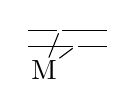
\begin{tikzpicture}[baseline=-.5em, inner sep=1pt, outer sep=0pt]
      \node (b1) at (.4,.1) {$\sbullet$};
      \node (b2) at (.6,-.1) {$\sbullet$};
      \draw (b1) -- (0, .1);
      \draw (b2) -- (0, -.1);
      \draw (b1) -- (1, .1);
      \draw (b2) -- (1, -.1);
      \node (M) at (.2,-.4) {M};
      \draw (M) -- (b1);
      \draw (M) -- (b2);
   \end{tikzpicture}
$
represents the tensor where $V_{i,j,i,j} = M_{i,j}$ and 0 otherwise.
So flattening $V$ on both sides is the same as $\mathrm{diag}(\mathrm{vec}(M))$,
which is the rhs of \eqref{eq:tensor_diag}.



\section{The Vec Operator}

The vec-operator applied on a matrix $A$ stacks the columns into a vector, i.e. for a $2\times 2$ matrix
\[
   \renewcommand*{\arraystretch}{1.3}
   A = \begin{bmatrix} A_{11} & A_{12} \\ A_{21} & A_{22} \end{bmatrix}
   \quad
   \mathrm{vec}(A) = \begin{bmatrix} A_{11} \\ A_{21} \\ A_{12} \\ A_{22} \end{bmatrix}
\]

At the start of the chapter we showed how to represent the vec-operator using the flattening tensor:
$
   \mathrm{vec}(X)
   =
   \begin{tikzpicture}[baseline=-.25em]
      \node (X) at (.5,0) {X};
      \node[triangle] (c0) at (1.5,0) {};
      \draw (X) edge[bend left] (c0);
      \draw (X) edge[bend right] (c0);
      \draw[double] (c0) -- ++(.5, 0);
   \end{tikzpicture}
$.
The Matrix Cookbook gives the following properties of the vec-operator:

\begin{align*}
   \tag{520}
   \mathrm{vec}(A^T X B)
   &=
   \mathrm{vec}(X)^T
   (A \otimes B)
                     &
   \begin{tikzpicture}[baseline=-.25em]
      \node (X) at (-.2,0) {X};
      \node (A) at (.5,.5) {A};
      \node (B) at (.5,-.5) {B};
      \node[triangle] (c1) at (1,0) {};
      \draw (X) -- (A) -- (c1);
      \draw (X) -- (B) -- (c1);
      \draw (c1) edge[double] ++(.5, 0);
   \end{tikzpicture}
                        &=
   \begin{tikzpicture}[baseline=-.25em]
      \node (X) at (.75,0) {X};
      \node[triangle] (c0) at (1.5,0) {};
      \node[triangle, rotate=180] (c1) at (2,0) {};
      \node (A) at (2.5,.5) {A};
      \node (B) at (2.5,-.5) {B};
      \node[triangle] (c2) at (3,0) {};
      \node (c3) at (3.4,0) {};
      \draw (X) edge[bend left] (c0);
      \draw (X) edge[bend right] (c0);
      \draw[double] (c0) -- (c1);
      \draw (c1) -- (A) -- (c2);
      \draw (c1) -- (B) -- (c2);
      \draw[double] (c2) -- (c3);
      % \draw [decorate,decoration={brace,amplitude=5pt,mirror,raise=4ex}]
      % (.5,-.75) -- (3.5,-.75) node[midway,yshift=-3em]{$\mathrm{vec}(X)^T(A \otimes B)$};
   \end{tikzpicture}
   \\
   \tag{521}
   \mathrm{Tr}(A^TB) &= \mathrm{vec}(A)^T \mathrm{vec}(B)
                     &
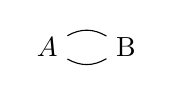
\begin{tikzpicture}[baseline=-.5em]
   \node (A) at (0,0) {$A$};
   \node (B) at (1,0) {B};
   \draw (A) edge[bend left] (B);
   \draw (A) edge[bend right] (B);
\end{tikzpicture}
&=
\begin{tikzpicture}[baseline=-.5em]
   \node (A) at (0,0) {A};
   \node (B) at (2,0) {B};
   \node[triangle] (c1) at (.66,0) {};
   \node[triangle, rotate=180] (c2) at (1.33,0) {};
   \draw (A) edge[bend left] (c1);
   \draw (A) edge[bend right] (c1);
   \draw (c1) edge[double] (c2);
   \draw (B) edge[bend left] (c2);
   \draw (B) edge[bend right] (c2);
\end{tikzpicture}
   \\
   \tag{522}
   \mathrm{vec}(A + B) &= \mathrm{vec}(A) +  \mathrm{vec}(B)
                       &
   \begin{tikzpicture}[baseline=-.25em]
      \node (a) at (0,0) {(A+B)};
      \node[triangle] (c1) at (1,0) {};
      \draw (c1) edge[double] ++(.4, 0);
      \draw (a) edge[bend left=10] (c1);
      \draw (a) edge[bend right=10] (c1);
   \end{tikzpicture}
                       &=
   \begin{tikzpicture}[baseline=-.25em]
      \node (a) at (0,0) {A};
      \node[triangle] (c1) at (.6,0) {};
      \draw (c1) edge[double] ++(.4, 0);
      \draw (a) edge[bend left=20] (c1);
      \draw (a) edge[bend right=20] (c1);
   \end{tikzpicture}
   +
   \begin{tikzpicture}[baseline=-.25em]
      \node (a) at (0,0) {B};
      \node[triangle] (c1) at (.6,0) {};
      \draw (c1) edge[double] ++(.4, 0);
      \draw (a) edge[bend left=20] (c1);
      \draw (a) edge[bend right=20] (c1);
   \end{tikzpicture}
   \\
   \tag{523}
   \mathrm{vec}(a A) &= a\, \mathrm{vec}(A)
                     &
   \begin{tikzpicture}[baseline=-.25em]
      \node (a) at (0,0) {$a A$};
      \node[triangle] (c1) at (.6,0) {};
      \draw (c1) edge[double] ++(.4, 0);
      \draw (a) edge[bend left=20] (c1);
      \draw (a) edge[bend right=20] (c1);
   \end{tikzpicture}
                     &=
   a
   \begin{tikzpicture}[baseline=-.25em]
      \node (a) at (0,0) {$A$};
      \node[triangle] (c1) at (.6,0) {};
      \draw (c1) edge[double] ++(.4, 0);
      \draw (a) edge[bend left=20] (c1);
      \draw (a) edge[bend right=20] (c1);
   \end{tikzpicture}
   \\
   \tag{524}
   a^T X B X^T c &= \mathrm{vec}(X)^T (B\otimes ca^T) \mathrm{vec}(X)
                 &
                 \vecmatvec{.5em}{a}{X,B,X}{c}
                 &=
   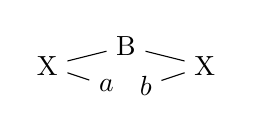
\begin{tikzpicture}[baseline=-.25em]
      \node (X1) at (2,0) {X};
      \node (B) at (3,.25) {B};
      \node (a) at (2.75,-.25) {$a$};
      \node (b) at (3.25,-.25) {$b$};
      \node (X2) at (4,0) {X};
      \draw (a) -- (X1) -- (B) -- (X2) -- (b);
   \end{tikzpicture}
               \\&&&=
   \begin{tikzpicture}[baseline=-.25em]
      \node (X) at (.75,0) {X};
      \node[triangle] (c0) at (1.5,0) {};
      \node[triangle, rotate=180] (c1) at (2,0) {};
      \node (A) at (2.75,.25) {B};
      \node (B1) at (2.5,-.25) {$a$};
      \node (B2) at (3,-.25) {$b$};
      \node[triangle] (c2) at (3.5,0) {};
      \node[triangle, rotate=180] (c3) at (4,0) {};
      \node (X1) at (4.75,0) {X};
      \draw (X) edge[bend left] (c0);
      \draw (X) edge[bend right] (c0);
      \draw (X1) edge[bend left] (c3);
      \draw (X1) edge[bend right] (c3);
      \draw[double] (c0) -- (c1);
      \draw (c1) -- (A) -- (c2);
      \draw (c1) -- (B1);
      \draw (B2) -- (c2);
      \draw[double] (c2) -- ++(.4,0);
   \end{tikzpicture}
\end{align*}

\section{General Matrification}

The last equation is an example of a general idea:
Any tensor network can be transformed into a series of matrix multiplications by applying the vec-operator to all tensors and the flattening tensor to all edges.
For example, the following complicated graph:
\begin{center}
   \def\svgwidth{.7\linewidth}
   \import{figures/}{kron.pdf_tex}
\end{center}
Can be written as a simple vector-matrix-matrix-vector product, $a M_1 M_2 b$,
where $M_1 = \mathrm{vec}(B) \otimes C'$,
$M_2 = E' \otimes D' \otimes I$ and $b = f\otimes g\otimes \mathrm{vec}(H)$,
where $C'$, $D'$ and $E'$ are rank 3 tensors flattened on one side, and $\mathrm{vec}(B)$ is interpreted as a matrix with a single column.


\subsection{The Lyapunov Equation}

A nice application of Kronecker product rewritings is to solve equations like
\begin{align*}
   \tag{272}
   AX + XB = C.
\end{align*}
We use the rewriting
$
   \mathrm{vec}(AX + XB)
   =
   (I \otimes A + B^T \otimes I)\mathrm{vec}(X)
$,
which follows from the tensor diagram massaging:
\[
\begin{tikzpicture}[baseline=-.25em]
   \node at (-1,0) {$\bigg($};
   \node at (-.75,0) {$+$};
   \node (A) at (0,.25) {A};
   \node (X1) at (.75,.25) {X};
   \node (X2) at (0,-.25) {X};
   \node (B) at (.75,-.25) {B};
   \node (br) at (1.5,0) {$\bigg)$};
   \draw (A) -- (X1) -- ++(.5,0);
   \draw (A) -- ++(-.5,0);
   \draw (X2) -- (B) -- ++(.5,0);
   \draw (X2) -- ++(-.5,0);
   \node[triangle] (f) at (2.2,0) {};
   \draw (br) edge[bend right] (f);
   \draw (br) edge[bend left] (f);
   \draw[double] (f) -- ++(.4,0);
\end{tikzpicture}
=
\begin{tikzpicture}[baseline=-.25em]
   \node (X) at (0,0) {X};
   \node (B) at (.65,.25) {A};
   \node[triangle] (f) at (1.1,0) {};
   \draw (X) edge[bend right] (f);
   \draw (X) -- (B) -- (f);
   \draw[double] (f) -- ++(.4,0);
\end{tikzpicture}
+
\begin{tikzpicture}[baseline=-.25em]
   \node (X) at (0,0) {X};
   \node (A) at (.65,-.25) {B};
   \node[triangle] (f) at (1.1,0) {};
   \draw (X) edge[bend left] (f);
   \draw (X) -- (A) -- (f);
   \draw[double] (f) -- ++(.4,0);
\end{tikzpicture}
=
   \begin{tikzpicture}[baseline=-.25em]
      \node (X) at (.75,0) {X};
      \node[triangle] (c0) at (1.5,0) {};
      \draw (X) edge[bend left] (c0);
      \draw (X) edge[bend right] (c0);
      \node (bl) at (2,0) {$\bigg($};
      \node at (2.25,0) {$+$};
      \draw[double, shorten <=-4pt] (bl) -- (c0);
      \node[triangle, rotate=180] (c1) at (3,.25) {};
      \node[triangle, rotate=180] (c2) at (3,-.25) {};
      \draw[double] (c1) -- ++(-.4,0);
      \draw[double] (c2) -- ++(-.4,0);
      \node (A) at (3.4,.4) {A};
      \node (B) at (3.4,-.4) {B};
      \node[triangle] (c3) at (3.8,.25) {};
      \node[triangle] (c4) at (3.8,-.25) {};
      \draw (c1) -- (A) -- (c3);
      \draw (c2) -- (B) -- (c4);
      \draw (c1) edge[bend right] (c3);
      \draw (c2) edge[bend left] (c4);
      \draw[double] (c3) -- ++(.4,0);
      \draw[double] (c4) -- ++(.4,0);
      \node (br) at (4.4,0) {$\bigg)$};
      \draw[double, shorten <=-6pt] (br) -- ++(.2,0);
   \end{tikzpicture}
\]
after which we can take the normal matrix inverse to get
\begin{align*}
   \tag{273}
   \mathrm{vec}(X) = (I \otimes A + B^T \otimes I)^{-1}\mathrm{vec}(C).
\end{align*}

\subsection{Encapsulating Sum}
This is a generalization of the previous equation.
\begin{align*}
   \tag{274}
   \sum_n A_nXB_n &= C \\
   \tag{275}
   \mathrm{vec}(X) &= (\sum_n B_n^T \otimes A_n)^{-1} \mathrm{vec}(C)
\end{align*}

\section{The Hadamard Product}

The Hadamard product, also known as element-wise multiplication, is not described in the Matrix Cookbook.
Yet, it is a very useful operation, and has some interesting properties in connection with the Kronecker product.

We define the Hadamard product of two $2\times 2$ matrices $A$ and $B$ as
\[
   \renewcommand*{\arraystretch}{1.3}
   A \circ B = \begin{bmatrix} A_{11} & A_{12} \\ A_{21} & A_{22} \end{bmatrix} \circ
              \begin{bmatrix} B_{11} & B_{12} \\ B_{21} & B_{22} \end{bmatrix}
            = \begin{bmatrix} A_{11}B_{11} & A_{12}B_{12} \\ A_{21}B_{21} & A_{22}B_{22} \end{bmatrix}
   .
\]
In tensor notation, the Hadamard product can be represented using two rank-3 copy tensors:
$
   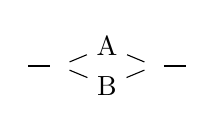
\begin{tikzpicture}[baseline=-.25em]
      \node (c0) at (0,0) {$\sbullet$};
      \node (A) at (.6,.25) {A};
      \node (B) at (.6,-.25) {B};
      \node (c1) at (1.2,0) {$\sbullet$};
      \draw (c0) -- (A) -- (c1);
      \draw (c0) -- (B) -- (c1);
      \draw (c0) -- ++(-.4,0);
      \draw (c1) -- ++(.4,0);
   \end{tikzpicture}
$.
Some properties of the Hadamard product are:
\begin{align*}
   x^T (A \circ B) y
   &= \mathrm{tr}(A^T D_x B D_y)
   &
   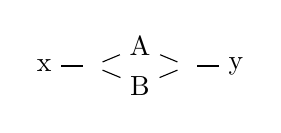
\begin{tikzpicture}[baseline=-.25em]
      \node (c0) at (0,0) {$\sbullet$};
      \node (A) at (.6,.25) {A};
      \node (B) at (.6,-.25) {B};
      \node (c1) at (1.2,0) {$\sbullet$};
      \draw (c0) -- (A) -- (c1);
      \draw (c0) -- (B) -- (c1);
      \draw (c0) -- ++(-.4,0) node[anchor=east] {x};
      \draw (c1) -- ++(.4,0) node[anchor=west] {y};
   \end{tikzpicture}
   &=
   \hspace{-2em}
   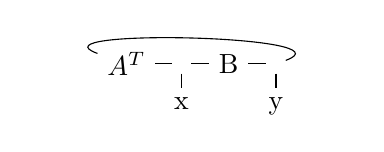
\begin{tikzpicture}[baseline=-.25em]
      \node (A) at (0,0) {$A^T$};
      \node (c0) at (.7,0) {$\sbullet$};
      \node (B) at (1.3,0) {B};
      \node (c1) at (1.9,0) {$\sbullet$};
      \draw (A) -- (c0) -- (B) -- (c1);
      \path (A) edge [out=160, in=20, looseness=1] (c1);
      \draw (c0) -- ++(0,-.3) node[anchor=north] {x};
      \draw (c1) -- ++(0,-.3) node[anchor=north] {y};
   \end{tikzpicture}
   \hspace{-2em}
   \\
   (A \otimes B)\circ(C \otimes D) &= (A\circ C) \otimes (B\circ D)
                                   &
   \begin{tikzpicture}[baseline=-.25em]
      \node (F0) at (0,0) {$\sbullet$};
      \node[triangle, rotate=180] (Fab0) at (.5,.5) {};
      \node (A) at (1,.75) {A};
      \node (B) at (1,.25) {B};
      \node[triangle] (Fab1) at (1.5,.5) {};
      \node[triangle, rotate=180] (Fcd0) at (.5,-.5) {};
      \node (C) at (1,-.25) {C};
      \node (D) at (1,-.75) {D};
      \node[triangle] (Fcd1) at (1.5,-.5) {};
      \node (F1) at (2,0) {$\sbullet$};
      \draw[double] (F0) -- ++(-.4,0);
      \draw[double] (F1) -- ++(.4,0);
      \draw[double] (F0) -- (Fab0);
      \draw[double] (Fab1) -- (F1);
      \draw[double] (F0) -- (Fcd0);
      \draw[double] (Fcd1) -- (F1);
      \draw (Fab0) -- (A) -- (Fab1);
      \draw (Fab0) -- (B) -- (Fab1);
      \draw (Fcd0) -- (C) -- (Fcd1);
      \draw (Fcd0) -- (D) -- (Fcd1);
   \end{tikzpicture}
                                   &=
   \begin{tikzpicture}[baseline=-.25em]
      \node[triangle, rotate=180] (F0) at (0,0) {};
      \node (Fab0) at (.5,.5) {$\sbullet$};
      \node (A) at (1,.75) {A};
      \node (B) at (1,.25) {B};
      \node (Fab1) at (1.5,.5) {$\sbullet$};
      \node (Fcd0) at (.5,-.5) {$\sbullet$};
      \node (C) at (1,-.25) {C};
      \node (D) at (1,-.75) {D};
      \node (Fcd1) at (1.5,-.5) {$\sbullet$};
      \node[triangle] (F1) at (2,0) {};
      \draw[double] (F0) -- ++(-.4,0);
      \draw[double] (F1) -- ++(.4,0);
      \draw (F0) -- (Fab0);
      \draw (Fab1) -- (F1);
      \draw (F0) -- (Fcd0);
      \draw (Fcd1) -- (F1);
      \draw (Fab0) -- (A) -- (Fab1);
      \draw (Fab0) -- (C.west);
      \draw (C.east) -- (Fab1);
      \draw (Fcd0) -- (B.west);
      \draw (B.east) -- (Fcd1);
      \draw (Fcd0) -- (D) -- (Fcd1);
   \end{tikzpicture}
\end{align*}
The first equation is simply massaging the tensor diagram.
The second follows from \eqref{eq:flatten_mix}.
Alternatively, it suffices to follow the double lines to see that $A$ and $C$ both use the ``upper'' part of the double edge, while $B$ and $D$ use the lower part.


\section{Khatri–Rao product}
Also known as the column-wise Kronecker, row-wise Kronecker or ``Face-splitting Product''.
We use the symbols $\ast$ and $\bullet$ for the column and row-wise Kronecker products, respectively.
\begin{align*}
   A \ast B &=
   \renewcommand*{\arraystretch}{1.3}
   \begin{bmatrix}
      A_{11} & A_{12} \\
      A_{21} & A_{22}
   \end{bmatrix}
   \ast
   \renewcommand*{\arraystretch}{1.3}
   \begin{bmatrix}
      B_{11} & B_{12} \\
      B_{21} & B_{22}
   \end{bmatrix}
            &=
   \renewcommand*{\arraystretch}{1.3}
   \begin{bmatrix}
      A_{11} B_{11} & A_{12} B_{12} \\
      A_{11} B_{21} & A_{22} B_{22} \\
      A_{21} B_{11} & A_{22} B_{12} \\
      A_{21} B_{21} & A_{22} B_{22}
   \end{bmatrix}
   \\
   A \bullet B &= \dots
            &=
   \renewcommand*{\arraystretch}{1.3}
   \begin{bmatrix}
      A_{11}  B_{11} & A_{11} B_{12} & A_{12} B_{11} & A_{12} B_{12} \\
      A_{21}  B_{21} & A_{21} B_{22} & A_{22} B_{21} & A_{22} B_{22}
   \end{bmatrix}
\end{align*}

In terms of tensor diagrams, these products correspond simply to flattening the product on one side, and using a copy tensor on the other:
\begin{align*}
   A \ast B &=
   \begin{tikzpicture}[baseline=-.25em]
      \node[triangle, rotate=180] (c0) at (0,0) {};
      \node (A) at (.6,.25) {A};
      \node (B) at (.6,-.25) {B};
      \node (c1) at (1.2,0) {$\sbullet$};
      \draw (c0) -- (A) -- (c1);
      \draw (c0) -- (B) -- (c1);
      \draw[double] (c0) -- ++(-.4,0);
      \draw (c1) -- ++(.4,0);
   \end{tikzpicture}
   \\
   A \bullet B &=
   \begin{tikzpicture}[baseline=-.25em]
      \node (c0) at (0,0) {$\sbullet$};
      \node (A) at (.6,.25) {A};
      \node (B) at (.6,-.25) {B};
      \node[triangle] (c1) at (1.2,0) {};
      \draw (c0) -- (A) -- (c1);
      \draw (c0) -- (B) -- (c1);
      \draw (c0) -- ++(-.4,0);
      \draw[double] (c1) -- ++(.4,0);
   \end{tikzpicture}
\end{align*}
Clearly the two are identical up to transpose.
Indeed, $(A \ast B)^T = B^T \bullet A^T$ and $(A \bullet B)^T = B^T \ast A^T$.

There are multiple ``mixed product'' identities:
\begin{align*}
   (A \bullet B)(C \otimes D) &= (A C) \bullet (B D)
                              &
   \begin{tikzpicture}[baseline=-.25em]
      \node (c0) at (0,0) {$\sbullet$};
      \draw (c0) -- ++(-.4,0);
      \node (A) at (.6,.25) {A};
      \node (B) at (.6,-.25) {B};
      \node[triangle] (c1) at (1.2,0) {};
      \draw (c0) -- (A) -- (c1);
      \draw (c0) -- (B) -- (c1);
      \node[triangle, rotate=180] (c2) at (1.7,0) {};
      \draw[double] (c1) -- (c2);
      \node (C) at (2.3,.25) {C};
      \node (D) at (2.3,-.25) {D};
      \node[triangle] (c3) at (2.9,0) {};
      \draw (c2) -- (C) -- (c3);
      \draw (c2) -- (D) -- (c3);
      \draw[double] (c3) -- ++(.4,0);
   \end{tikzpicture}
                              &=
   \begin{tikzpicture}[baseline=-.25em]
      \node (c0) at (0,0) {$\sbullet$};
      \node (A) at (.6,.25) {A};
      \node (B) at (.6,-.25) {B};
      \node (C) at (1.2,.25) {C};
      \node (D) at (1.2,-.25) {D};
      \node[triangle] (c1) at (1.8,0) {};
      \draw (c0) -- (A) -- (C) -- (c1);
      \draw (c0) -- (B) -- (D) -- (c1);
      \draw (c0) -- ++(-.4,0);
      \draw[double] (c1) -- ++(.4,0);
   \end{tikzpicture}
   \\
   (A x) \circ (B y) &= (A \bullet C) (x \otimes y)
                     &
   \begin{tikzpicture}[baseline=-.25em]
      \node (c0) at (0,0) {$\sbullet$};
      \draw (c0) -- ++(-.4,0);
      \node (A) at (.6,.25) {A};
      \node (B) at (.6,-.25) {B};
      \node (x) at (1.2,.25) {x};
      \node (y) at (1.2,-.25) {y};
      \draw (c0) -- (A) -- (x);
      \draw (c0) -- (B) -- (y);
   \end{tikzpicture}
                     &=
   \begin{tikzpicture}[baseline=-.25em]
      \node (c0) at (0,0) {$\sbullet$};
      \draw (c0) -- ++(-.4,0);
      \node (A) at (.6,.25) {A};
      \node (B) at (.6,-.25) {B};
      \node[triangle] (c1) at (1.2,0) {};
      \draw (c0) -- (A) -- (c1);
      \draw (c0) -- (B) -- (c1);
      \node[triangle, rotate=180] (c2) at (1.7,0) {};
      \draw[double] (c1) -- (c2);
      \node (x) at (2.3,.25) {x};
      \node (y) at (2.3,-.25) {y};
      \draw (c2) -- (x);
      \draw (c2) -- (y);
   \end{tikzpicture}
\end{align*}


\subsection{Stacking}
Can be part of Kronecker section

From Josh:
Proposition 2.5. For any field $\mathbb{F}$, integers $d_1, d_2, d_3, d_4$ and matrices $X_1 \in \mathbb{F}^{d_1 \times d_2}, X_2 \in \mathbb{F}^{d_2 \times d_3}$, $X_3 \in \mathbb{F}^{d_1 \times d_4}$, and $X_4 \in \mathbb{F}^{d_4 \times d_3}$, we have
$$
X_1 \times X_2+X_3 \times X_4=\left(X_1 \mid X_3\right) \times\left(\frac{X_2}{X_4}\right),
$$
where we are writing '|'to denote matrix concatenation.

With tensor diagrams we can write stacking along a new axis $i$ as
\[
\mathrm{stack}_i(X, Y)
=
\begin{tikzpicture}[baseline=-.5em, inner sep = 1pt]
    \node (e) at (0, .2) {$e^{(0)}$};
    \draw (e) -- ++(.5,0) node[midway, above right, font=\tiny] {$i$};
    \node (X) at (0, -.2) {$X$};
    \draw (X) -- ++(.5,0);
    \draw (X) -- ++(-.5,0);
\end{tikzpicture}
+
\begin{tikzpicture}[baseline=-.5em, inner sep = 1pt]
    \node (e) at (0, .2) {$e^{(1)}$};
    \draw (e) -- ++(.5,0) node[midway, above right, font=\tiny] {$i$};
    \node (X) at (0, -.2) {$Y$};
    \draw (X) -- ++(.5,0);
    \draw (X) -- ++(-.5,0);
\end{tikzpicture}
\]
where $e^{(i)}_i=1$ and 0 elsewhere.

Fro this we easily get the identity
\begin{align}
\left(A \mid C\right) \left(\frac{B}{D}\right)
&=
\mathrm{stack}_i(A, C)
\,
% \times_i
\mathrm{stack}_i(B, D)
\\&=
\left(
\begin{tikzpicture}[baseline=-.5em, inner sep = 1pt]
    \node (e) at (0, .2) {$e^{(0)}$};
    \draw (e) -- ++(.5,0) node[midway, above right, font=\tiny] {$i$};
    \node (X) at (0, -.2) {$A$};
    \draw (X) -- ++(-.5,0) node[midway, below left, font=\tiny] {$k$};
    \draw (X) -- ++(.5,0) node[midway, below right, font=\tiny] {$j$};
\end{tikzpicture}
+
\begin{tikzpicture}[baseline=-.5em, inner sep = 1pt]
    \node (e) at (0, .2) {$e^{(1)}$};
    \draw (e) -- ++(.5,0) node[midway, above right, font=\tiny] {$i$};
    \node (X) at (0, -.2) {$C$};
    \draw (X) -- ++(-.5,0) node[midway, below left, font=\tiny] {$k$};
    \draw (X) -- ++(.5,0) node[midway, below right, font=\tiny] {$j$};
\end{tikzpicture}
\right)
\left(
\begin{tikzpicture}[baseline=-.5em, inner sep = 1pt]
    \node (e) at (0, .2) {$e^{(0)}$};
    \draw (e) -- ++(.5,0) node[midway, above right, font=\tiny] {$i$};
    \node (X) at (0, -.2) {$B$};
    \draw (X) -- ++(-.5,0) node[midway, below left, font=\tiny] {$j$};
    \draw (X) -- ++(.5,0) node[midway, below right, font=\tiny] {$m$};
\end{tikzpicture}
+
\begin{tikzpicture}[baseline=-.5em, inner sep = 1pt]
    \node (e) at (0, .2) {$e^{(1)}$};
    \draw (e) -- ++(.5,0) node[midway, above right, font=\tiny] {$i$};
    \node (X) at (0, -.2) {$D$};
    \draw (X) -- ++(-.5,0) node[midway, below left, font=\tiny] {$j$};
    \draw (X) -- ++(.5,0) node[midway, below right, font=\tiny] {$m$};
\end{tikzpicture}
\right)
\\&=
\begin{tikzpicture}[baseline=-.5em, inner sep = 1pt]
    \node (e) at (0, .2) {$e^{(0)}$};
    \draw (e) -- ++(.5,0);
    \node (X) at (0, -.2) {$A$};
    \draw (X) -- ++(.5,0);
    \draw (X) -- ++(-.5,0) node[midway, below left, font=\tiny] {$k$};
\end{tikzpicture}
\,
\begin{tikzpicture}[baseline=-.5em, inner sep = 1pt]
    \node (e) at (0, .2) {$e^{(0)}$};
    \draw (e) -- ++(-.5,0);
    \node (X) at (0, -.2) {$B$};
    \draw (X) -- ++(.5,0) node[midway, below right, font=\tiny] {$m$};
    \draw (X) -- ++(-.5,0);
\end{tikzpicture}
+
\begin{tikzpicture}[baseline=-.5em, inner sep = 1pt]
    \node (e) at (0, .2) {$e^{(1)}$};
    \draw (e) -- ++(.5,0);
    \node (X) at (0, -.2) {$C$};
    \draw (X) -- ++(.5,0);
    \draw (X) -- ++(-.5,0) node[midway, below left, font=\tiny] {$k$};
\end{tikzpicture}
\,
\begin{tikzpicture}[baseline=-.5em, inner sep = 1pt]
    \node (e) at (0, .2) {$e^{(1)}$};
    \draw (e) -- ++(-.5,0);
    \node (X) at (0, -.2) {$D$};
    \draw (X) -- ++(.5,0) node[midway, below right, font=\tiny] {$m$};
    \draw (X) -- ++(-.5,0);
\end{tikzpicture}
\\&=
AB + CD
\end{align}

TODO: Relation to direct sum, which is basically stacking + flattening.
Or maybe it's nicer to do it by hadamard producting with the $e_i$ vector.
Also notice that this is what quantum comp people call ``controlling''.

Also have a bunch of properties like $A\otimes(B\oplus C) = A\otimes B\oplus A\otimes C$.


\section{Exercises}
\begin{exercise}
Let $
J = \mathrm{Tr}\lbrack(I_N \otimes F)^{T}A(I_N \otimes F)B\rbrack
$ where $F \in \mathbb{R}^{N \times Nn},\ \  A \in \mathbb{R}^{N^2 \times N^2},\ B \in \mathbb{R}^{N^2 n \times N^2 n}$.
Find the derivative of $J$ with respect to $F$.
\end{exercise}


\begin{exercise}
Consider $ J = \|G - ( B \otimes X )\|_F^2 $, where $G$ and $B$ are matrices, and $\|\cdot\|_F$ is the Frobenius norm. Find the derivative with respect to $X$
\end{exercise}

\begin{exercise}
Prove the equation~\cite{2993406}:
\[\text{vec}(A\, \text{diag}(b)\, C)=((C^T\otimes 1) \circ (1 \otimes A)) b.\]
Here $\text{diag}(b)$ is a diagonal matrix with the vector $b$ on the diagonal, $1$ is a vector of ones of the right size, and $b \otimes A$, the Kronecker product for a vector and a matrix, is defined by $\begin{tikzpicture}[baseline=-.25em, inner sep=0pt]
      \node[triangle, rotate=180, inner sep=3pt] (flat) at (0,0) {};
      \node (A) at (.5,-.15) {$A$};
      \node (B) at (.5,.15) {$b$};
      \draw[double] (flat) -- ++(-.4,0);
      \draw (flat) -- (A) -- ++(.4,0);
      \draw (flat) -- (B);
   \end{tikzpicture}$,
that is, you just flatten on one side.
\end{exercise}

\begin{exercise}
   Let $a$ and $b$ be two vectors and let $D$ and $X$ be two matrices.
   Minimize the following cost function with respect to $X$:
   \[
      E = \|a - D X b\|_2^2.
   \]
\end{exercise}

\begin{exercise}
   Prove using diagrams that $\mathrm{Tr}(A^T B) = 1^T \mathrm{vec}(A \circ B)$,
   where $1$ is a vector of the appropriate size.
\end{exercise}

\begin{exercise}
   Find the derivative of
   \[
      \mathrm{Tr}(G(A\otimes X))
   \]
   with respect to $X$.
\end{exercise}

\begin{exercise}
   % TODO: Find tag name
   \[\frac{\partial}{\partial \mathbf{X}} \operatorname{Tr}(\mathbf{X} \otimes \mathbf{X})=\frac{\partial}{\partial \mathbf{X}} \operatorname{Tr}(\mathbf{X}) \operatorname{Tr}(\mathbf{X})=2 \operatorname{Tr}(\mathbf{X}) \mathbf{I}\]
\end{exercise}
